\chapter{Optimal coordinated axial induction control of a wind-farm boundary layer}\label{ch:opt_induction}
This chapter discusses a first optimization study in which the methodology of previous chapter is applied. The current chapter is a continuation of earlier work on optimal coordinated axial induction control of wind farms presented in \cite{goit2015optimal} and \cite{goit2016optimal}. Here, we consider the optimal control of a wind farm with 72 turbines arranged in an aligned layout. Similarities and differences of the current study with the preceding works are highlighted throughout the chapter. The current chapter focuses on the case definition and observation of the optimal control results in terms of increased power extraction and differences in the wind-farm flow. Further, the influence of the wind-turbine response time defined in Section~\ref{sec:meth_adm} on thrust loading variability and power extraction is investigated. An in-depth analysis of the control mechanisms of the current case, with the aim of gaining physical insights useful towards the development of practical controllers, will be presented later in Chapter~\ref{ch:opt_analysis}. 

The outline of the chapter is as follows. Section~\ref{sec:opt_ind_setup} describes the cases considered here, and elucidates numerical setup details. Section~\ref{sec:opt_ind_results} discusses the results of the optimal control simulations. Concluding, Section~\ref{sec:opt_ind_summ} summarizes the key aspects of this chapter. 

Parts of the content of this chapter have been published in the following articles:
\begin{itemize}
	\item \cite{munters2016effect}, ``Effect of wind turbine response time on optimal dynamic induction control of wind farms'', \emph{Journal of Physics: Conference Series} \textbf{753}, 052007
	\item \cite{munters2017optimal}, ``An optimal control framework for dynamic induction control of wind farms and their interaction with the atmospheric boundary layer'', \emph{Phil. Trans. R. Soc. A} \textbf{375}, 20160100
\end{itemize}

\section{Numerical setup and case description}\label{sec:opt_ind_setup}
In the current chapter, we consider a wind farm consisting of 72 turbines with hub height $z_h = 100$ m and a rotor diameter $D = 100$ m. Turbines are arranged in a $12 \times 6$ aligned pattern, and are spaced apart by 6 rotor diameters in axial and transversal directions. Firstly, the optimization problem at hand is detailed. Secondly, the numerical setup for the simulation and optimization is elaborated. Finally, a set of control cases is defined. 

\subsubsection{Optimization problem}
The optimal control studies in the current chapter consider dynamic induction without yawing, i.e. wind turbines remain aligned with the mean flow direction throughout the simulation. In this case $\omega_{\rm max} = 0$, and the optimization problem from Chapter~\ref{ch:opt_formulation} can be simplified, resulting in the following problem:
\begin{mini!}[1]
	{\scriptsize \bs{\varphi}, \bs{q}}{\J(\bs{\varphi}, \bs{q}) = - \Tint \sum_{i=1}^{N_t} \frac{1}{2} a \ctihat~V_i^3 A_i \dt}{\label{eq:indcostfunction_inside_problem}}{}
	%	\addConstraint{\small \frac{\partial \utilde}{\partial t} + \big(\utilde \cdot \nabla \big)\utilde }{\small = - \nabla (\ptilde + \ptilde_\infty) / \rho - \nabla \cdot \boldsymbol{\tau}_{sgs} + \sum_{i=1}^{N_t} \bs{f}_i\ + \bs{f}_{\text{fr}} }{\small \text{in } \Omega \times (0,T] \label{eq:NSmomentum_constraint}}
	\addConstraint{\small \frac{\partial \utilde}{\partial t} + \big(\utilde \cdot \nabla \big)\utilde }{\small = - \nabla \ptilde / \rho - \nabla \cdot \boldsymbol{\tau}_{sgs} + \sum_{i=1}^{N_t} \bs{f}_i\ + \bs{f}_{\text{fr}}\ \ }{\small \text{in } \Omega \times (0,T] \label{eq:indNSmomentum_constraint}}	
	\addConstraint{\small \nabla \cdot \utilde}{\small =0, \label{eq:indNScontinuity_constraint}}{\small \text{in } \Omega \times (0,T]}
	\addConstraint{\small \tau \ddt{\ctihat}}{\small =\cti - \ctihat \label{eq:indctihat_constraint}}{\small i=1...N_t~\text{in } (0,T]}
	\addConstraint{\small C_{T,\text{min}}' \leq}{\small  \cti \leq C_{T,\text{max}}' \label{eq:indboxct_constraint}}{\small i=1...N_t~\text{in } (0,T]}
\end{mini!}
with states $\bs{q}(\bs{x},t) = [\ufilt(\bs{x},t),\ \ptilde(\bs{x},t),\ \widehat{\bs{C}}_T'(t)]$ and controls $\bs{\varphi}(t)~=~\bs{C}_T'(t)$. The numerical values for $C_{T, \rm min}'$ and $\ctmax$ in the box constraints are given in Table~\ref{tab:setup_params_ind}.

\subsubsection{Simulation setup}
The wind-farm boundary layer is simulated on a spatial domain of $10 \times 3.6 \times 1$ km$^3$, discretized using a grid of $384 \times 192 \times 244$ gridpoints. A driving pressure gradient of $\partial_x p_\infty/\rho = 2.5 \times 10^{-4}$ m s$^{-2}$ results in a free-stream hub-height velocity slightly over 8 m s$^{-1}$. Figure~\ref{fig:domain} illustrates a typical snapshot of the LES velocity field for the wind farm considered here. It can be seen from the figure that, starting from the second row, turbines are subjected to significantly lower velocities with increased variability. Moreover, it is shown that the LES allows to capture complex unsteady wake behavior, including meandering and turbulent entrainment, that can potentially be harnessed by the optimal control approach. Unsteady turbulent inflow conditions are the same for all cases, and are generated using the database precursor method from Section~\ref{sec:inflow_CP} with a precursor simulation of identical dimensions as the main simulation. The precursor simulation uses the shifted periodic boundary conditions from Section~\ref{sec:inflow_shifted} to generate fully-developed turbulent inflow.  

Wind farm operation is optimized over $N_A = 15$ receding-horizon time windows (see Section~\ref{sec:problem_receding}), resulting in a total time of $T_{tot} = N_AT_A = 30$ minutes. Time integration is performed using a constant timestep $\Delta t = 0.75$ s. We employ a prediction horizon of $T = 240$ s, and a flow advancement horizon of $T_A = T/2 = 120$ s. Based on numerical experiments, we retain $m = 5$ correction pairs for the BFGS Hessian updates. This proved to be an adequate parameter choice, both here and for a varied set of constrained problems in the CUTE collection \citep{bongartz1995cute}, as illustrated in \cite{byrd1995limited}. To limit the overall computational expense, we stop the optimization algorithm after $N_{it} = 60$ iterations. As further shown below, this leads to approximately 120 PDE evaluations (forward or adjoint), with a total walltime of about 24 hours per window on 320 Intel Ivy Bridge processor cores connected by a QDR Infiniband network. The ratio between physical control time and computational walltime is hence approximately 1 : 700, a significant reduction compared to 1 : 1800 in the case of \cite{goit2015optimal} and \cite{goit2016optimal}. Furthermore, as will be shown in this chapter, the current study performs more iterations, higher power gains and better converged results than the former works. The initial guess for the optimal controls is a steady $C_T' = 2$ for all turbines, corresponding to greedy Betz-optimal behavior (see discussion below). Simulation and optimization parameters are summarized in Table~\ref{tab:setup_params_ind}. 

Simulations are initialized as follows: firstly, a fully-developed high-Reynolds number turbulent boundary layer is generated by simulating a perturbed logarithmic flow over a physical timespan of approximately 36 hours. Subsequently, wind turbines are inserted in the simulation, and the flow field is advanced in time for approximately 5 wind-farm flow-through times, after which the effects of any wind-farm start-up transients have subsided in the main domain. This wind-farm boundary layer in statistically stationary state is used as initial condition for all simulation cases, and the corresponding time is set as $t = 0$~s in the remainder of this work.

\begin{figure}
	\centering
	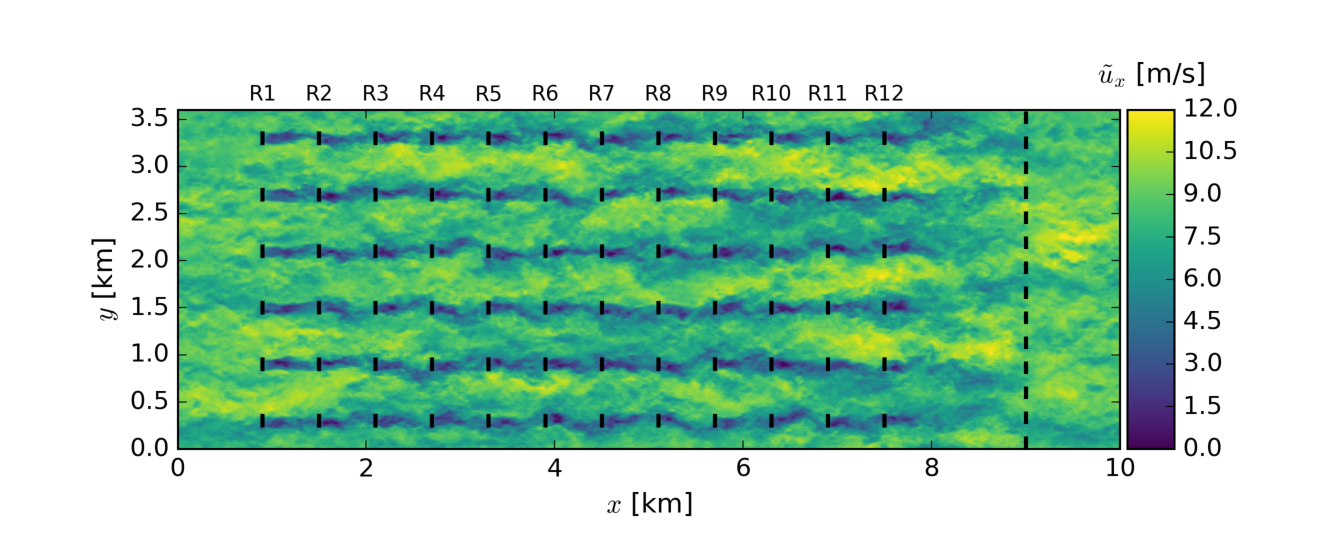
\includegraphics[width=\linewidth]{chapters/philtrans_torque/figure6.eps}
	\caption[Large-eddy simulation streamwise velocity field for a 12 $\times$ 6 aligned wind farm.]{Large-eddy simulation streamwise velocity field for a 12 $\times$ 6 aligned wind farm. The black lines represent the turbine rotors. The black dashed line indicates the start of the fringe region for imposition of turbulent inflow conditions (see Section~\ref{sec:meth_fringe}).}
	\label{fig:domain}
\end{figure}

\begin{table}[t]	
	\caption{Setup parameters for optimal dynamic induction control cases}\label{tab:setup_params_ind}
	\centering
	\begin{tabular}{ll}
		\hline \\
		\textbf{Simulation parameters} & \\
		Domain size  & 			$L_x \times L_y \times H = (9 \boldsymbol{+1}) \times 3.6 \times 1$ km$^3$  \\ 
		Driving pressure gradient  & 	$ \partial_x p_\infty = 2.5 \times 10^{-4}$ m s$^{-2}$  \\ 
		Turbine dimensions  &  $D = 0.1H = 100$ m, \quad $z_h = 0.1H = 100$ m\\ 
		Turbine spacing  &  $S_x = 6D, \quad S_y = 6D$\\
		Wind-farm layout & $N_t = 72 $ turbines = 12 rows $\times$ 6 columns \\ 
		Surface roughness  &  $z_0 = 10^{-4}H = 0.1$m\\ 
		Grid size & $N_x \times N_y \times N_z = 384 \times 256 \times 144$\\
		Cell size & $\Delta_x \times \Delta_y \times \Delta_z = 26 \times 14 \times 6.9$ m$^3$\\
		Time step & $\Delta t = 0.75$ s\\		
		&\\
		\textbf{Optimization parameters} & \\ 
		Optimization method			& L-BFGS-B \\
		Hessian correction pairs 	& $m = 5$ \\
		BFGS iterations 			& $N_{it} = 60$ ($\approx 120$ PDE) \\
		Optimization time window					& $T = 240$ s\\
		Flow advancement time window & $T_A = 120$ s\\
		Total operation time         & $T_{tot} = 1800$ s (15 windows)\\
		&\\
		\textbf{Cases} & \\
		R			& $C_T' = 2$\\
		C3t0		& $0 \leq C_T' \leq 3$  \quad   $\tau = 0$ s (overinductive)\\
		C3t5		& $0 \leq C_T' \leq 3$  \quad   $\tau = 5$ s (overinductive)\\
		C3t30		& $0 \leq C_T' \leq 3$  \quad   $\tau = 30$ s (overinductive)\\
		C2t0		& $0 \leq C_T' \leq 2$  \quad   $\tau = 0$ s (underinductive)\\			C2t5		& $0 \leq C_T' \leq 2$  \quad   $\tau = 5$ s (underinductive)\\
		C2t30		& $0 \leq C_T' \leq 2$  \quad   $\tau = 30$ s (underinductive)\\		
		\hline 
	\end{tabular} 
\end{table}

\subsubsection{Control cases}

We consider a reference case (R) in which turbines greedily maximize individual power by setting their thrust coefficients to a steady Betz-optimal value $C_T' = 2$.  In addition, we define a set of optimal control cases in which thrust coefficient setpoints $\widehat{C}_T'$ are varied dynamically for each wind turbine. As shown in Figure~\ref{fig:under_overinductive}, momentum theory indicates that, for every desired $C_P < 16/27$ (i.e. the Betz limit), two possible $C_T'$ setpoints can be found: an \emph{underinductive} setpoint $C_T' < 2$, and an \emph{overinductive} setpoint $C_T' > 2$. By modifying $\ctmax$, we can hence define different control cases, based upon whether overinduction is allowed ($\ctmax = 3$, see Section~\ref{sec:meth_adm}), or not ($\ctmax = 2$). Further, we aim to quantify the influence of smoothness of the thrust coefficient $\cthat$ on the resulting power gains and thrust force dynamics. This is done by selecting the WT response time as $\tau = 0$, $5$, or $30$ s for an instantaneous, fast, or slow response respectively. This is in contrast to previous work, which only considered instantaneous wind-turbine response \citep{goit2015optimal,goit2016optimal}. The response of the thrust coefficient $\cthat$ to a step variation in the setpoint $C_T'$ is illustrated in Figure~\ref{fig:cthat_ind}. Note however that control setpoints originating from the optimal control will be much more complex.  

\begin{figure}[t]
	\centering
	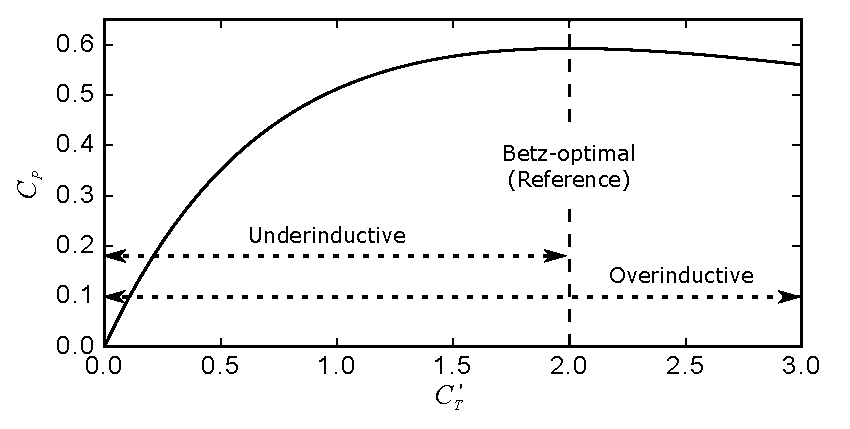
\includegraphics[width=0.75\linewidth]{figures/meth_ct_ctprime_cp2.eps}
	\caption{Illustration of reference, underinductive ($C_{T,\text{max}}' = 2$) and overinductive ($C_{T,\text{max}}' = 3$) cases on momentum theory-based power coefficient curve.\label{fig:under_overinductive}}
\end{figure}

\begin{figure}[t]
	\centering
	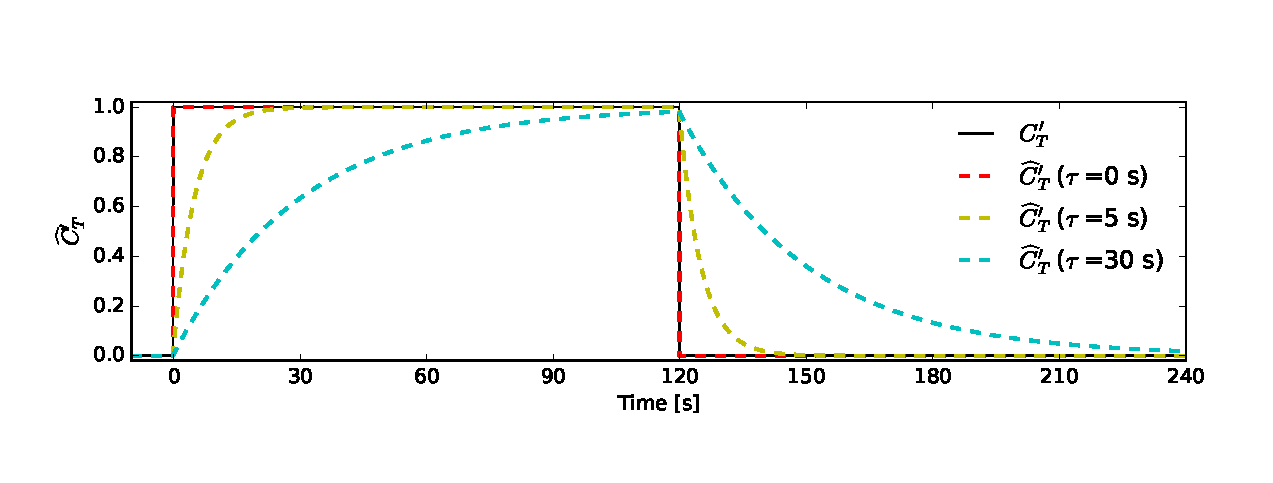
\includegraphics[width=\textwidth]{chapters/optimal_control_problem/figure3.eps}    
	\caption{Illustration of the response of the thrust coefficient $\widehat{C}_T'$ to a square wave variation in the control signal $C_T'$ for varying wind turbine response times $\tau$. \label{fig:cthat_ind}}
\end{figure}
 
In summary, this leads to the definition of 6 optimal axial induction control cases: a set of overinductive cases and a set of underinductive cases, both of which contain an instantaneous, fast, and slow response case. Optimal control cases are denoted as C<X>t<Y>, where X and Y represent $\ctmax$ and $\tau$ respectively, e.g. C3t30 for the case with $\ctmax=3$ and $\tau=30$ s. The definition of the control cases is summarized in Table~\ref{tab:setup_params_ind}.

%------------------------------------------
% Table setup parameters
%------------------------------------------
%\begin{table}[p]


\section{Optimal coordinated control results}\label{sec:opt_ind_results}
This section discusses the optimization results using the setup mentioned above. Firstly, we put the results into context by investigating the convergence behavior and sensitivity to the initial control guess $\bs{\varphi}_0$. Thereafter, Section~\ref{sec:opt_ind_energy} discusses the gains in energy extraction achieved by the optimal control simulations. Subsequently, Section~\ref{sec:opt_ind_dyn} illustrates the turbine dynamics on the level of control settings and thrust forces in order to accomplish these gains. Lastly, Section~\ref{sec:opt_ind_flow} depicts the differences in flow field statistics between the reference and controlled cases.

Figure~\ref{fig:window_opt} illustrates the convergence behavior for all optimal control simulations. From Figure~\ref{fig:window_opt}a it can be seen that, for most cases, the amount of PDE evaluations is only slightly higher than twice the amount of BFGS iterations $N_{it}$, illustrating that the optimization algorithm mostly takes steps with unit length, and only rarely has to resort to a line search when $\alpha$ does not satisfy the Wolfe conditions introduced in Section~\ref{sec:problem_optimization}. Note that case C2t30 achieved convergence after 120 iterations, with a large increase in PDE simulations in the preceding iterations. This indicates that, upon approaching convergence, inconsistencies between the gradient obtained from the continuous adjoint approach and the actual cost functional gradient are making it harder to satisfy the Wolfe conditions, and more line searches are needed. This behavior also starts to show in the later iterations of the other cases. Figure~\ref{fig:window_opt}b depicts the relative improvement in the cost function within an optimization window in terms of the amount of iterations. It can be seen that, after 60 iterations, the improvement rate of the cost function significantly decreases. Figure~\ref{fig:window_opt}c shows the cost functional as a function of PDE evaluations. The circle markers indicate the datapoints for which $N_{it} = 60$. The figure shows that all cases achieve reasonable convergence for the chosen iteration limit, i.e. further improvements of the cost functional are minimal. These observations justify terminating the optimization after 60 iterations for the cases described in this chapter. 

\begin{figure}
	\centering
	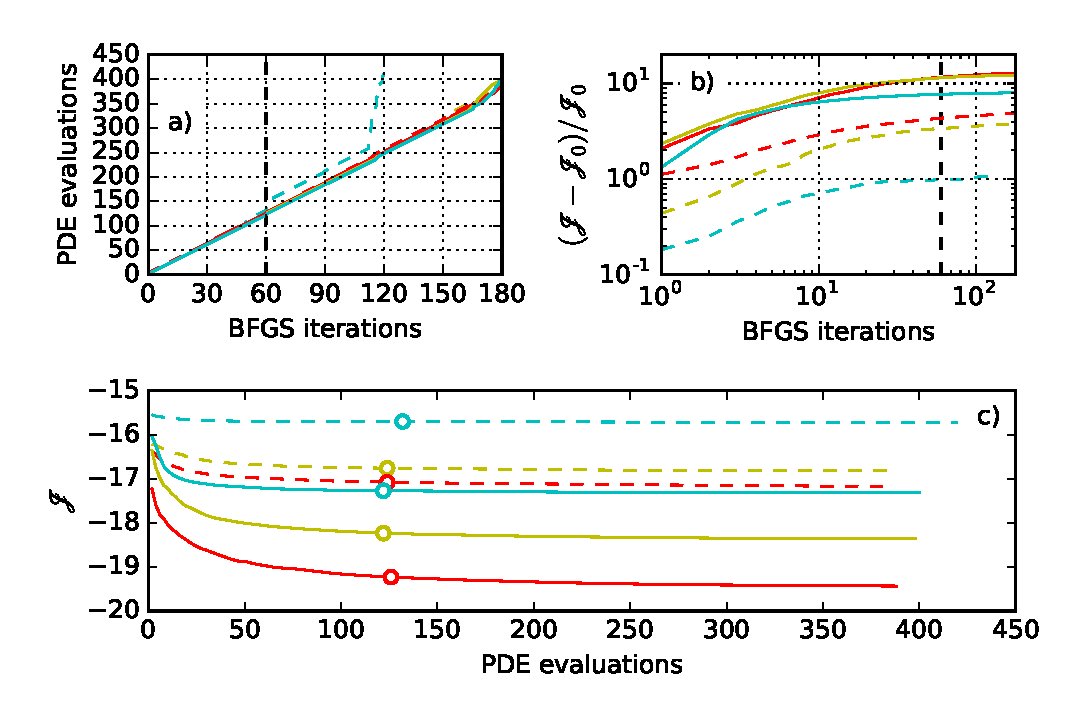
\includegraphics[width=0.9\linewidth]{chapters/philtrans_torque/figure11.eps}
	\caption[Convergence behavior for the third optimization window.]{Convergence behavior for the third optimization window. (Legend: \legendnoref) \label{fig:window_opt}}
\end{figure}
	
Given the non-convexity of the Navier--Stokes constrained optimization problems considered here, the cost functional landscape is expected to be characterized by a multitude of local optima. Figure~\ref{fig:initial_conditions} shows the cost functional and a subset of the optimized controls for different starting points $\blds{\varphi}_0$, i.e. a greedy control case on the one hand, for which all turbines operate Betz-optimal at $\blds{\varphi}_0 = [2 \ \ 2 \ \dots \ 2]$, and a case with $\blds{\varphi}_0 = [1.33 \ \ 1.33 \ \dots \ 1.33]$ on the other hand. Figure~\ref{fig:initial_conditions}a illustrates cost functional decrease in terms of BFGS iterations. It can be seen that the choice of initial conditions has only a minor influence on the power extraction. Figure~\ref{fig:initial_conditions}b shows the optimized controls for the first row of the wind farm after 1, 60, 120, and 180 iterations. Although some regions of the controls are similar for both initial conditions, mainly at the start of the optimization window the controls differ significantly. Since the overall energy extraction seems only modestly dependent on the initial condition, the greedy control with $\varphi_0 = 2$ is a suitable starting point for wind-farm optimal control.

\begin{figure}[ht!]
	\centering
	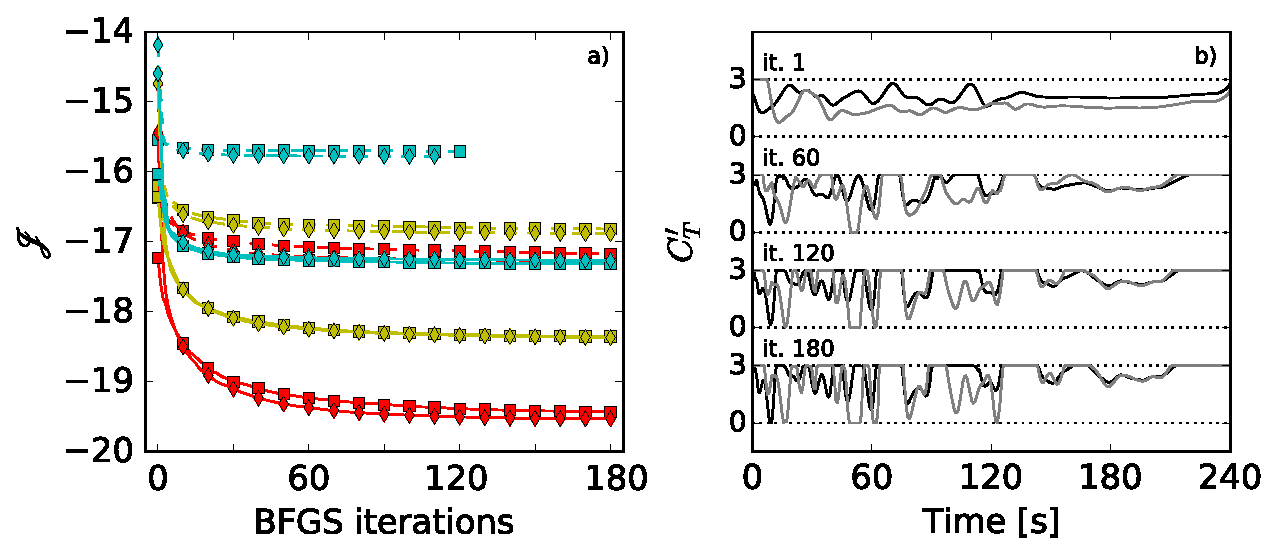
\includegraphics[width=\linewidth]{chapters/philtrans_torque/figure13.eps}	
	\caption[Sensitivity of optimization to initial conditions.]{Sensitivity of optimization to initial conditions. \emph{a):} Cost functional as a function of BFGS iterations for a single window. ($\square$: $\blds{\varphi}_0 = 2$, $\lozenge$: $\blds{\varphi}_0 = 1.33$, \legendnoref ). \emph{b):} Optimized controls for a front row turbine at various iterations. (Black: $\blds{\varphi}_0 = 2$, Gray: $\blds{\varphi}_0 = 1.33$). \label{fig:initial_conditions}} 
\end{figure}


\subsection{Wind-farm energy extraction}\label{sec:opt_ind_energy}

Figure~\ref{fig:bar_and_row} depicts the energy extraction of the optimally controlled wind farms normalized by the reference case. The energy extraction is integrated starting from the second optimization window, since the optimized wind farms are still in a transient phase during the first window. It is shown in Figure~\ref{fig:bar_and_row}a that all cases, except for the most restrictive case C2t30, achieve significant energy gains ranging between 8 and 21\%. This illustrates the potential of dynamic coordinated control approaches over greedy individual control. As can be expected, decreasing flexibility with regards to $C_T'^{max}$ and $\tau$ reduces the margins for increased power extraction. It is worth noting that the slow-response overinductive case C3t30 achieves power gains close to the underinductive fast-response cases C2t0 and C2t5. This observation is promising for the eventual actual roll-out of dynamic wind farm controllers, as it shows that fast temporal variations in turbine control settings, with associated detrimental effects on turbine structural loading, are not a prerequisite for significant improvements in power extraction. The error bars in the figure indicate two standard deviations from the sampled mean. Error estimates are within $\pm 1.2$\% points for all cases except C3t0, for which $\pm 1.9$\% points is observed. The variances of relative energy gains are estimated using variances and covariances defined on the optimization window level, as further elaborated in Appendix~\ref{ch:app_variance}. In Figure~\ref{fig:bar_and_row}b it is shown that energy extraction is increased in every downstream row. The first row slightly downrates the first row for all cases except C3t30. Moreover, the first row aside, the last row extracts the most energy for all cases, since it does not have to take into account any downstream neighbors. Note that the cases considered here feature significantly larger energy gains than the comparable case in \cite{goit2016optimal}, for which an increase in energy extraction of approximately 6\% was reported. This directly results from the updates to the optimization framework discussed throughout this thesis: the combination of the improved solver parallelization as discussed in Section~\ref{sec:meth_par} with the updated quasi-Newton optimizer from Section~\ref{sec:problem_optimization} allow us to run more cases with better convergence within a reasonable time to solution. Moreover, the better convergence obtained in the current simulation set will allow us to perform more detailed analysis of the flow field statistics and control dynamics, as will be shown later in this text.

\begin{figure}
	\centering
	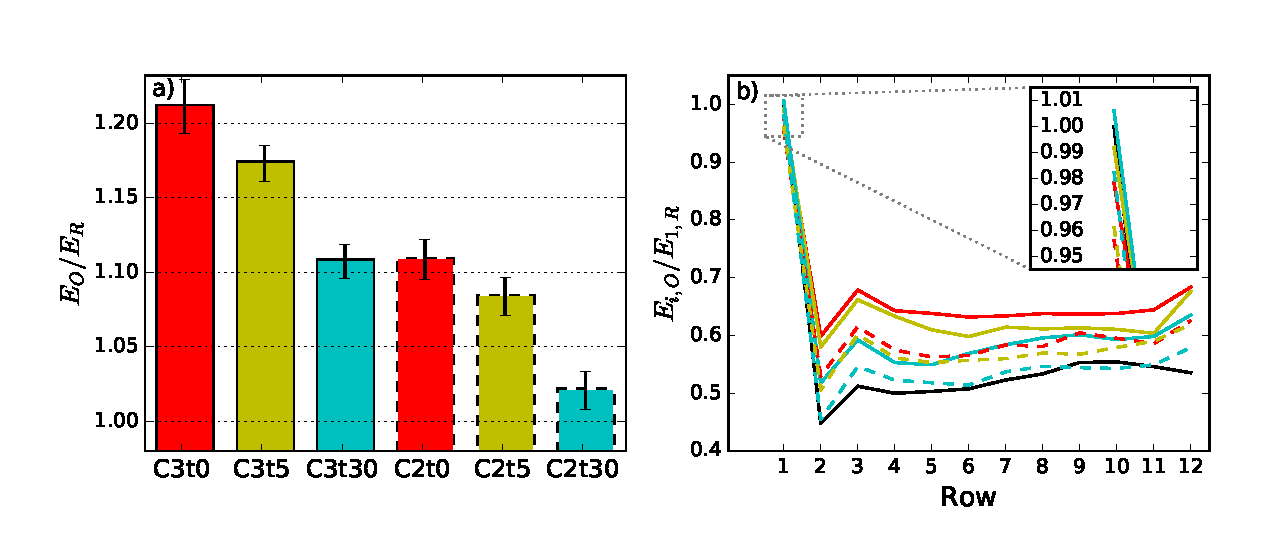
\includegraphics[width=\linewidth]{chapters/philtrans_torque/figure8.eps}
	\caption[Energy extraction of optimally controlled wind farms $E_O$ normalized by greedy reference case $E_R$.]{Energy extraction of optimally controlled wind farms $E_O$ normalized by greedy reference case $E_R$. \emph{a) } Total energy extraction. Error bars indicate confidence intervals of $\pm 2$ standard deviations. \emph{b) } Energy extraction per row, normalized by first row of reference case. \legend \label{fig:bar_and_row}}
\end{figure}

\subsection{Wind-farm dynamics}\label{sec:opt_ind_dyn}
Figure~\ref{fig:time_control_and_time_power} illustrates the dynamic behavior for all cases over 30 minutes of operation time. Figures~\ref{fig:time_control_and_time_power}a and~\ref{fig:time_control_and_time_power}c depict a front-row turbine thrust coefficient setpoint $C_T'$ and its time-filtered counterpart $\widehat{C}_T'$ for the overinductive and underinductive cases respectively. It can be seen from these figures that $C_T'$ varies wildly between its upper and lower bound in response to the turbulent dynamics of the boundary layer, and that time-filtering greatly reduces temporal variability in $\widehat{C}_T'$. Figures~\ref{fig:time_control_and_time_power}b and~\ref{fig:time_control_and_time_power}d show the total power extraction normalized by reference power. We see for all cases that optimal control leads to an increase in temporal variations of extracted power, and that time-filtering significantly reduces potentially harmful variability on shorter time scales. The periodic variations on longer time scales that can be observed for all cases except C2t30 are caused by finite-horizon optimization effects.
We note that C2t30 hardly differs from the reference case R, with $\widehat{C}_T' \approx 2$ for virtually all turbines throughout the entire time horizon. This indicates that, for underinductive control of the considered wind-farm setup, variations on shorter time scales are essential for significant power increase through optimal control. Further analysis of the optimized controls and the physical mechanisms behind increasing power extraction will be presented in Chapter~\ref{ch:opt_analysis}. 

\begin{figure}
	\centering
	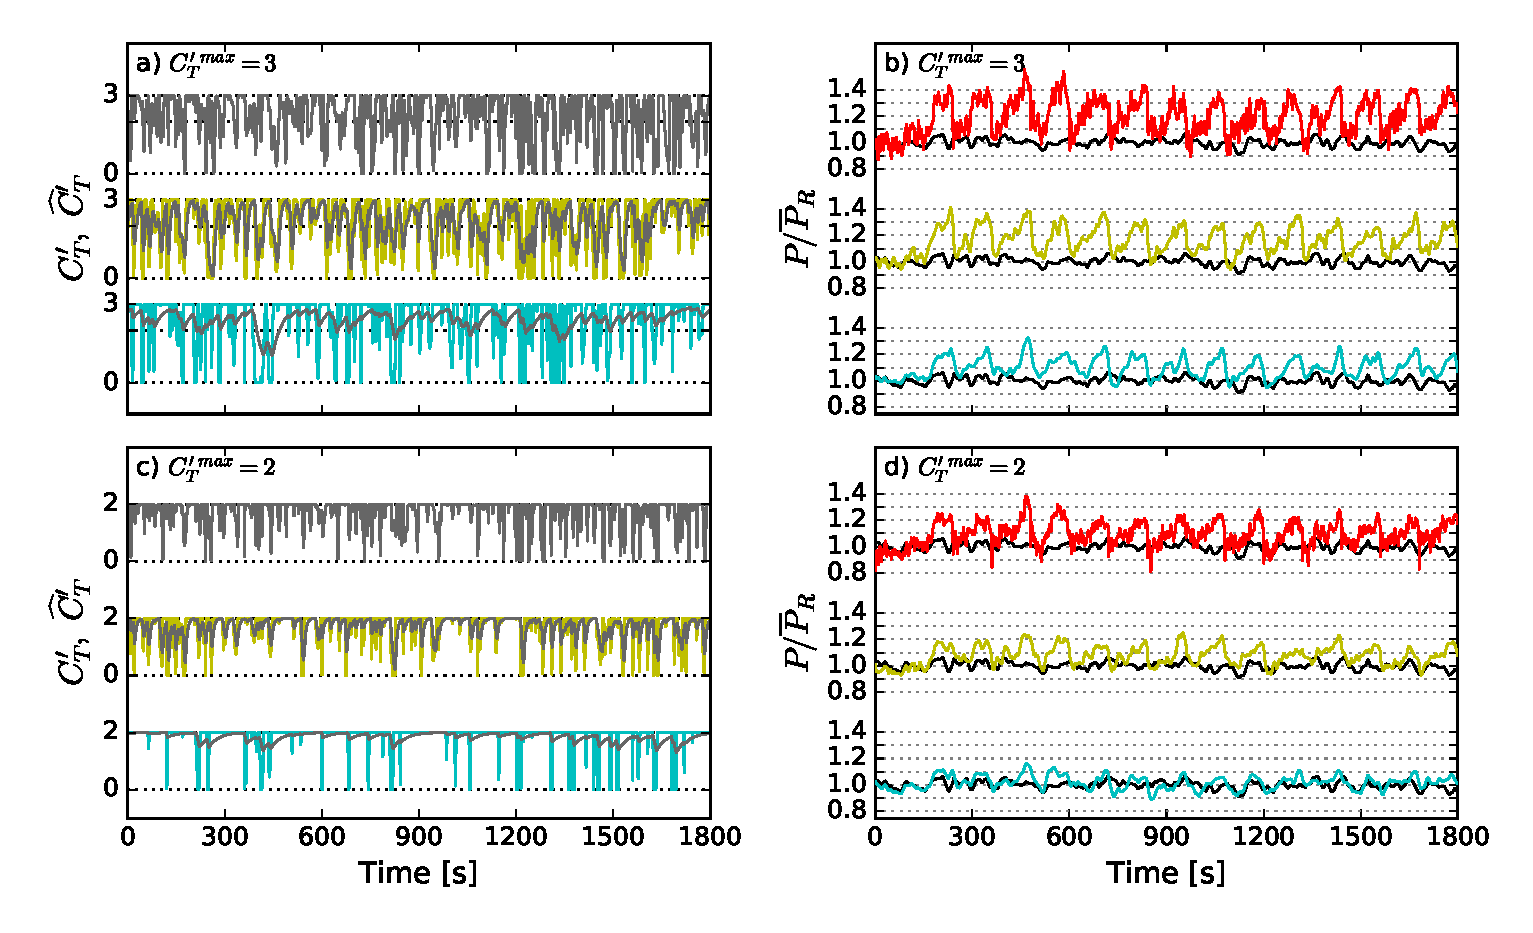
\includegraphics[width=0.93\linewidth]{chapters/philtrans_torque/dynamics.eps}
	\caption[Temporal behavior of optimally controlled wind farms.]{Temporal behavior of optimally controlled wind farms. 
		\emph{Left (a,c): } Thrust coefficient of the wind turbine in the first row of the central column. Colors: setpoint coefficient $C_T'$, Grey: time-filtered coefficient $\widehat{C}_T'$. \emph{Right (b,d): } Aggregate power extraction normalized by time average of reference power extraction. \emph{Top (a,b): } $C_T'^{max}=3$. \emph{Bottom (c,d): } $C_T'^{max} = 2$. \legendtauref \label{fig:time_control_and_time_power}}
\end{figure}

Figure~\ref{fig:thrust} shows the dynamic behavior of the thrust force $f_t$ for a turbine $t$ in row 6 of the wind farm, where turbulence levels at hub height approach a fully-developed state. Figure~\ref{fig:thrust}a illustrates the time series of $f_t$, normalized by the time-averaged values of the same turbine in the reference case. It can be seen that case C3t0 exhibits high frequency force variations and peak forces regularly exceeding values twice as large as the time average reference $\overline{f}_{t,R}$. Such high-frequency, high-amplitude load cycling can significantly reduce wind-turbine lifetime through fatigue, and is hence to be avoided. Cases C3t5 and C3t30 show that increasing response time $\tau$ not only filter out high frequency force fluctuations, but also leads to a reduction of the largest force amplitudes for this wind turbine. A further decrease in amplitudes is achieved by reducing $C_T'^{max}$ to 2. Figure~\ref{fig:thrust}b shows the power spectra of the time series illustrated in~\ref{fig:thrust}a. Low frequency behavior ($\leq 10^{-2}$ Hz) is similar for all cases and tends to a --1 slope, indicating that the slowest force variations are governed by the background atmospheric dynamics. Around $10^{-2}$ Hz, a small --5/3 range is observed. At higher frequencies, a slope between --3 and --4 characterizes the controlled cases,  while the static reference case decays much more quickly. In this range, the turbine response time to variations in control setpoint directly translates to the frequency content of the thrust force enacted by the turbine. It is important to note that, not only should fatigue be taken into account when considering additional cyclic turbine loading due to dynamic wind farm control, also natural frequencies of relevant deformation modes should be avoided at all cost. For example, the natural frequency associated with the tower fore-aft deformation mode of the NREL 5 MW turbine is approximately 0.3 Hz \citep{jonkman2009definition}. It can be seen from Figure~\ref{fig:thrust} that cases C3t0 and C2t0 show significant spectral energy in this range. These results indicate that a detailed analysis of turbine structural loading, through the addition of a multi-physics aero-elastic turbine model in the governing equations is an essential step towards actual rollout of fast-response dynamic wind farm controllers. This is an important topic for future research.

\begin{figure}
	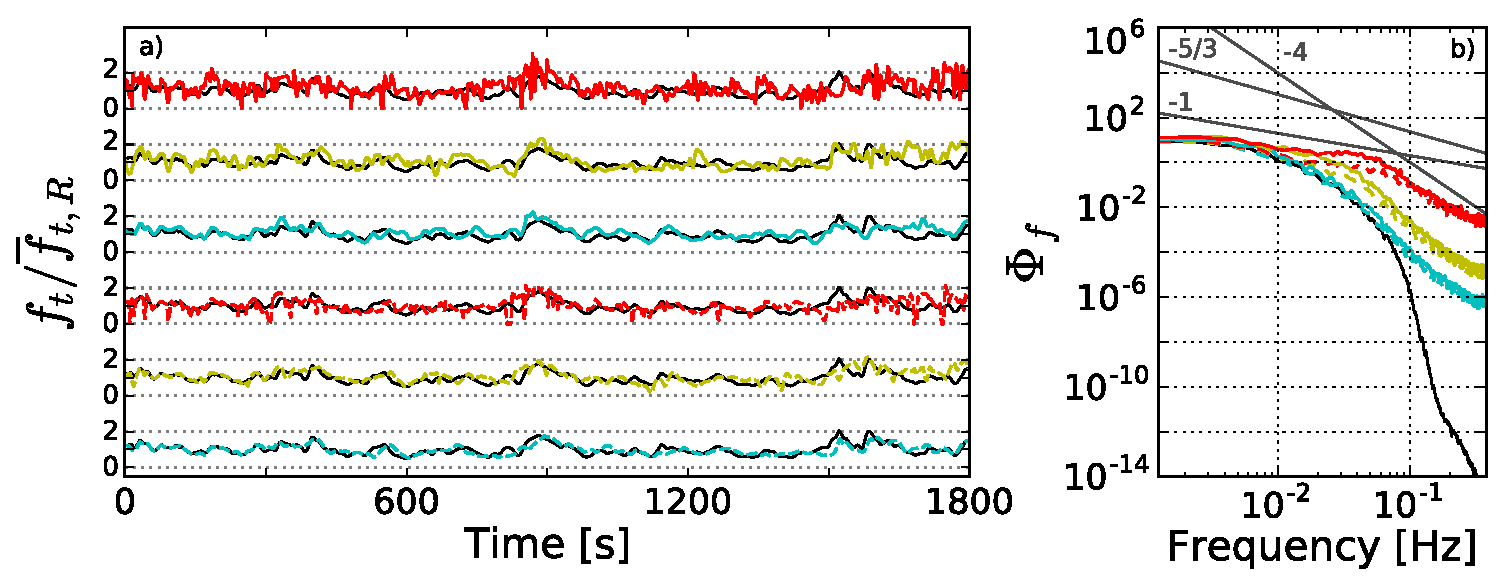
\includegraphics[width=\textwidth]{chapters/philtrans_torque/thrust_forces.eps}
	\caption[Dynamic behavior of thrust force $f_t$ for the wind turbine in the central column of the sixth row.]{Dynamic behavior of thrust force $f_t$ for the wind turbine in the central column of the sixth row. \emph{a)} Time series of thrust force, normalized by time-averaged reference thrust. \emph{b) } Power spectra $\Phi_f$ of normalized thrust force, averaged over columns. \legend \label{fig:thrust}}
\end{figure}




\subsection{Wind-farm flow field statistics}\label{sec:opt_ind_flow}

	Here, we discuss the differences in time-averaged flow field statistics between the reference case and the optimal control cases. For sake of brevity, we focus on the four cases with the highest power extraction, i.e. the overinductive cases C3t0, C3t5, and C3t30, and the instantaneous underinductive case C2t0. Moreover, the flow field is averaged over six spanwise domain slabs, associated with each of the turbine columns. Firstly, axial velocity is discussed as the main driver behind wind-farm power extraction. Thereafter, kinetic energy, and transversal and vertical transport of axial momentum are illustrated. In the following discussion, a standard Reynolds decomposition of the velocity is applied, defining the time-averaged mean velocity $\widetilde{U} \equiv \overline{\widetilde{u}}$ and the turbulent fluctuating velocity $\widetilde{u}' \equiv  \widetilde{u} - \widetilde{U}$.

	\subsubsection{Mean axial velocity}

	Figures~\ref{fig:opt_ind_top_u} and~\ref{fig:opt_ind_side_u} respectively show planviews at hub height and sideviews through the rotor
	centerline of time-averaged axial velocity ${\widetilde{U}}_x$. It can be seen from both figures that, for all cases, downstream
	turbines are subjected to higher incoming flow velocities. The overinductive cases show a larger drop in $\widetilde{U}_x$ over the
	rotor disk, most notably in the first row turbines, indicating relatively deeper wakes with enhanced recovery before hitting the next row of
	turbines. In contrast, this larger drop is not observed for the underinductive case C2t0: the lower average $\cthat$ causes shallower averaged
	wakes throughout the entire wind farm. Further, it can be observed that, for the overinductive cases, the axial velocity in the flow above and
	besides the wind turbine column is reduced, indicating that these regions are depleted of mean-flow kinetic energy. This is further discussed
	below. This reduction is visible to a much lesser extent in the underinductive case C2t0.
	
	% TOPVIEW U
	\begin{figure}[ht]
		\centering
		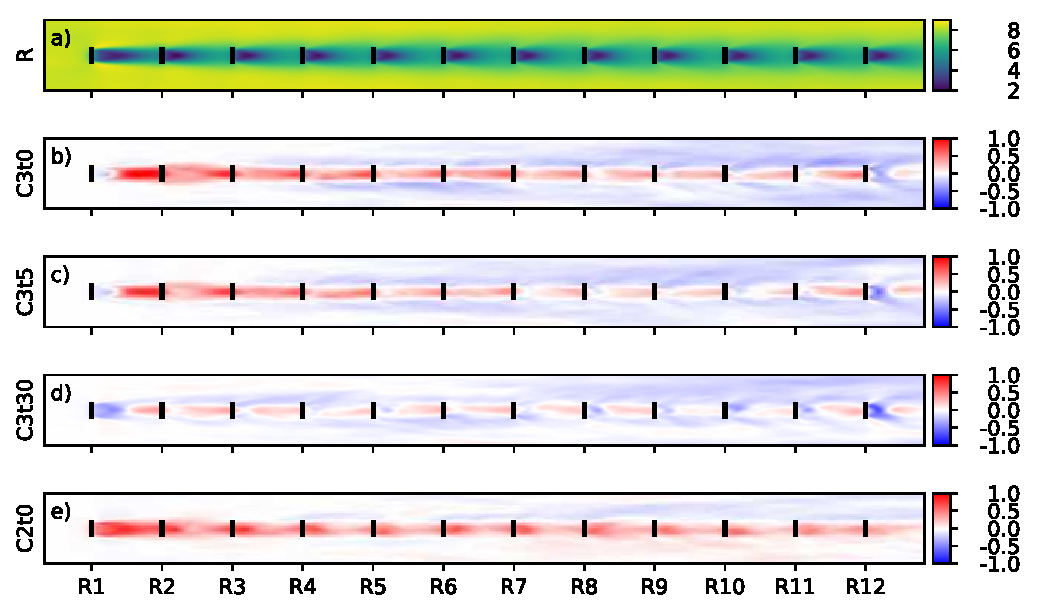
\includegraphics[width=0.93\textwidth]{chapters/optimal_induction_control/topview_u.eps}
		\caption[Planview ($xy$) of time-averaged axial velocity $\widetilde{U}_x$ at hub height.]{Planview ($xy$) of time-averaged axial velocity $\widetilde{U}_x$ at hub height. \emph{a) } Reference case. \emph{b-e)} Difference between optimal control cases and reference case, defined as $\Delta = \widetilde{U}_{x,\text{opt}} - \widetilde{U}_{x,\text{R}}$  \label{fig:opt_ind_top_u}}
	\end{figure}

	% SIDEVIEW U
	\begin{figure}[hbt]
		\centering
		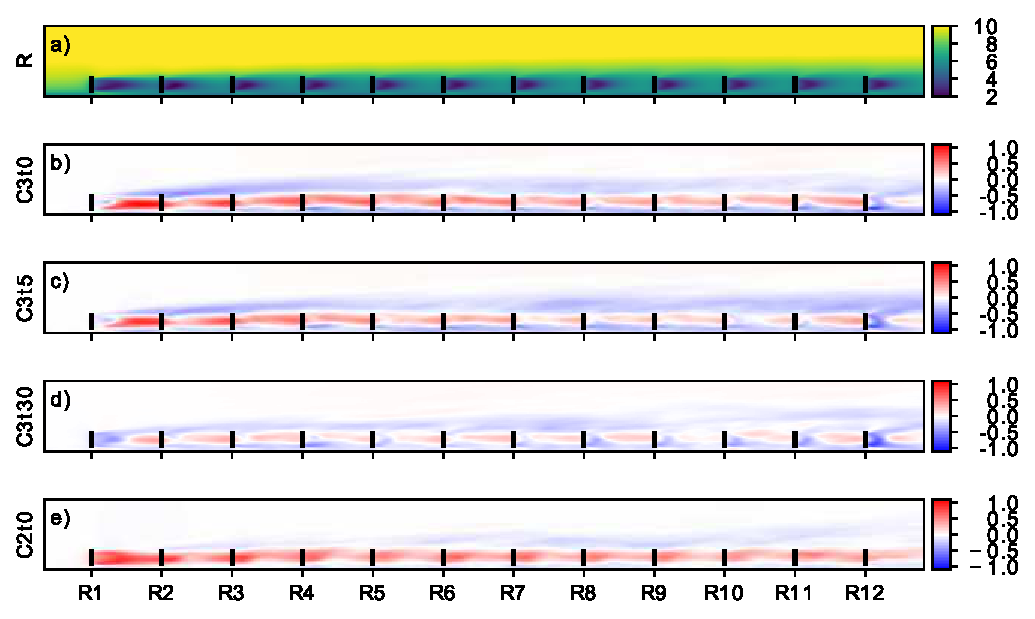
\includegraphics[width=0.93\textwidth]{chapters/optimal_induction_control/sideview_u.eps}
		\caption[Sideview ($xz$) of time-averaged axial velocity $\widetilde{U}_x$ in turbine centerline plane.]{Sideview ($xz$) of time-averaged axial velocity $\widetilde{U}_x$ in turbine centerline plane. \emph{a) } Reference case. \emph{b-e)} Difference between optimal control cases and reference case, defined as $\Delta = \widetilde{U}_{x,\text{opt}} - \widetilde{U}_{x,\text{R}}$  \label{fig:opt_ind_side_u}}
	\end{figure}	
	
	
	\subsubsection{Kinetic energy}

	Figures~\ref{fig:opt_ind_top_u} and~\ref{fig:opt_ind_side_u} respectively show planviews at hub height and sideviews through the rotor
	centerline of \emph{total} kinetic energy KE = $(\overline{\widetilde{u}_x \widetilde{u}_x} + \overline{\widetilde{u}_y \widetilde{u}_y} + \overline{\widetilde{u}_z \widetilde{u}_z})/2$. Focusing on the overinductive cases C3t0 and C3t5, it can be observed that, in the entrance region of the wind farm, mainly the internal boundary layer above the turbines gets depleted of kinetic energy by the optimal control (see Figure~\ref{fig:opt_ind_side_total_ke}b,c). The same effect can be observed in cases C3t30 and C2t0, but to a far lesser extent. Returning to C3t0 and C3t5, it is shown that, as the flow progresses downstream, this effect subsides somewhat, and also the intercolumn channels besides the turbines lose some kinetic energy (see Figure~\ref{fig:opt_ind_top_total_ke}b,c). 

		% SIDEVIEW KE
		\begin{figure}[ht]
			\centering
			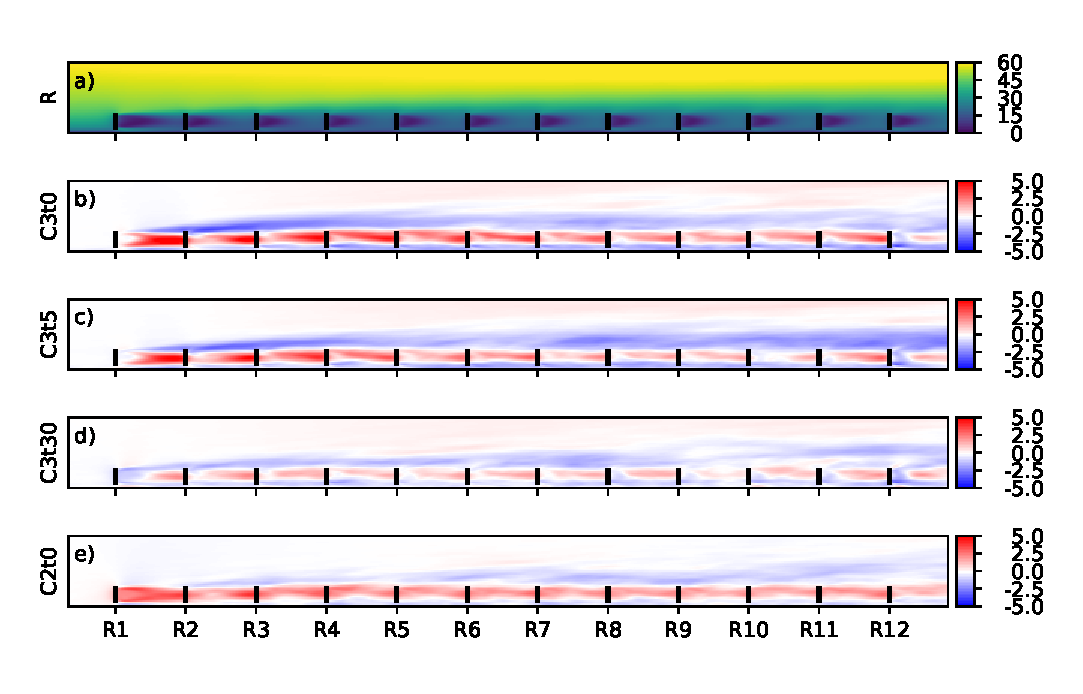
\includegraphics[width=0.93\textwidth]{chapters/optimal_induction_control/sideview_ke_total_side.eps}
			\caption[Sideview ($xz$) of \emph{total} kinetic energy KE $= (\overline{\widetilde{u}_x \widetilde{u}_x} + \overline{\widetilde{u}_y \widetilde{u}_y} + \overline{\widetilde{u}_z \widetilde{u}_z})/2$ in turbine centerline plane.]{Sideview ($xz$) of \emph{total} kinetic energy KE $= (\overline{\widetilde{u}_x \widetilde{u}_x} + \overline{\widetilde{u}_y \widetilde{u}_y} + \overline{\widetilde{u}_z \widetilde{u}_z})/2$ in turbine centerline plane. \emph{a) } Reference case. \emph{b-e)} Difference between optimal control and reference case, defined as $\Delta = \text{KE}_{\text{opt}} - \text{KE}_{R}$  \label{fig:opt_ind_side_total_ke}}
		\end{figure}

		% SIDEVIEW KE
		\begin{figure}[hbt]
			\centering
			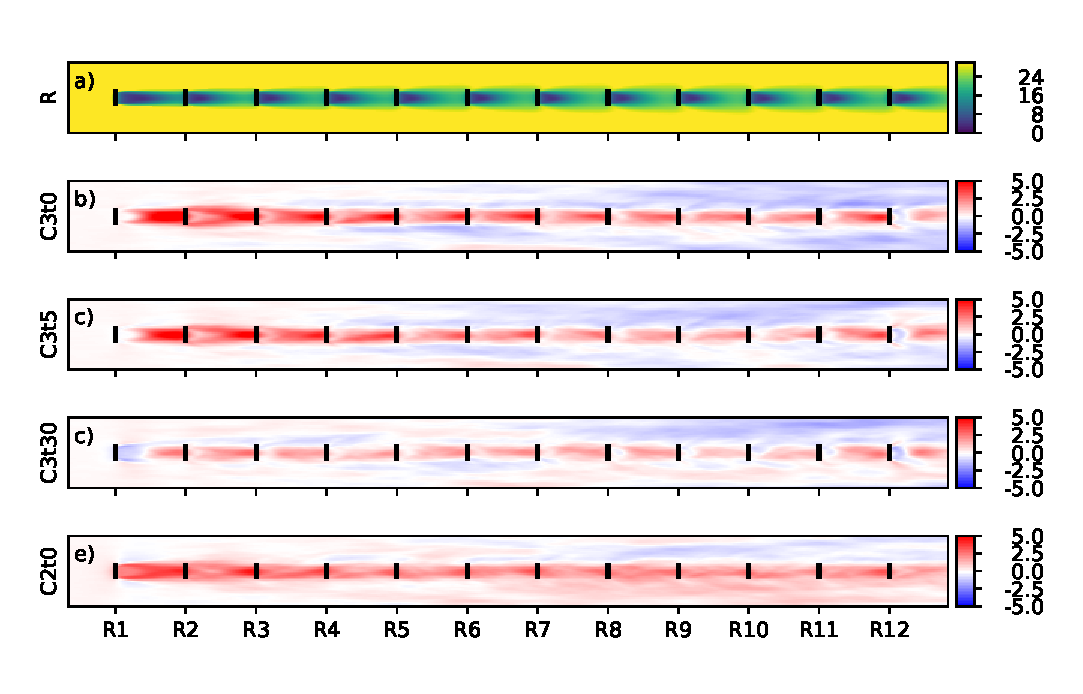
\includegraphics[width=0.93\textwidth]{chapters/optimal_induction_control/topview_ke_total.eps}
			\caption[Planview ($xy$) of \emph{total} kinetic energy KE $= (\overline{\widetilde{u}_x \widetilde{u}_x} +
			\overline{\widetilde{u}_y \widetilde{u}_y} + \overline{\widetilde{u}_z \widetilde{u}_z})/2$ in hub height.]{Planview ($xy$) of \emph{total} kinetic energy KE $= (\overline{\widetilde{u}_x \widetilde{u}_x} +
			\overline{\widetilde{u}_y \widetilde{u}_y} + \overline{\widetilde{u}_z \widetilde{u}_z})/2$ in hub height. \emph{a) } Reference case. \emph{b-e)} Difference between optimal control and reference case, defined as $\Delta = \text{KE}_{\text{opt}} - \text{KE}_{R}$  \label{fig:opt_ind_top_total_ke}}
		\end{figure}
	
		Figures~\ref{fig:opt_ind_top_tke} and~\ref{fig:opt_ind_side_tke} show planviews and sideviews of \emph{turbulence} kinetic energy $k = (\overline{\widetilde{u}_x'\widetilde{u}_x'} + \overline{\widetilde{u}_y'\widetilde{u}_y'} + \overline{\widetilde{u}_z'\widetilde{u}_z'})/2$. The overinductive cases show an increase in turbulence throughout the entire wind farm, spreading to the internal boundary layer above the turbines and the intercolumn channels alongside them in the downstream regions of the wind farm. Note specifically the sharp increase in $k$ in the core wake regions behind the first rows of case C3t0 and C3t5. Contrastingly, the underinductive case C2t0 shows less coherent behavior, except for a slight turbulence increase in the near wake of the first-row turbines.
	
		% TOPVIEW TKE	
		\begin{figure}[ht]
			\centering
			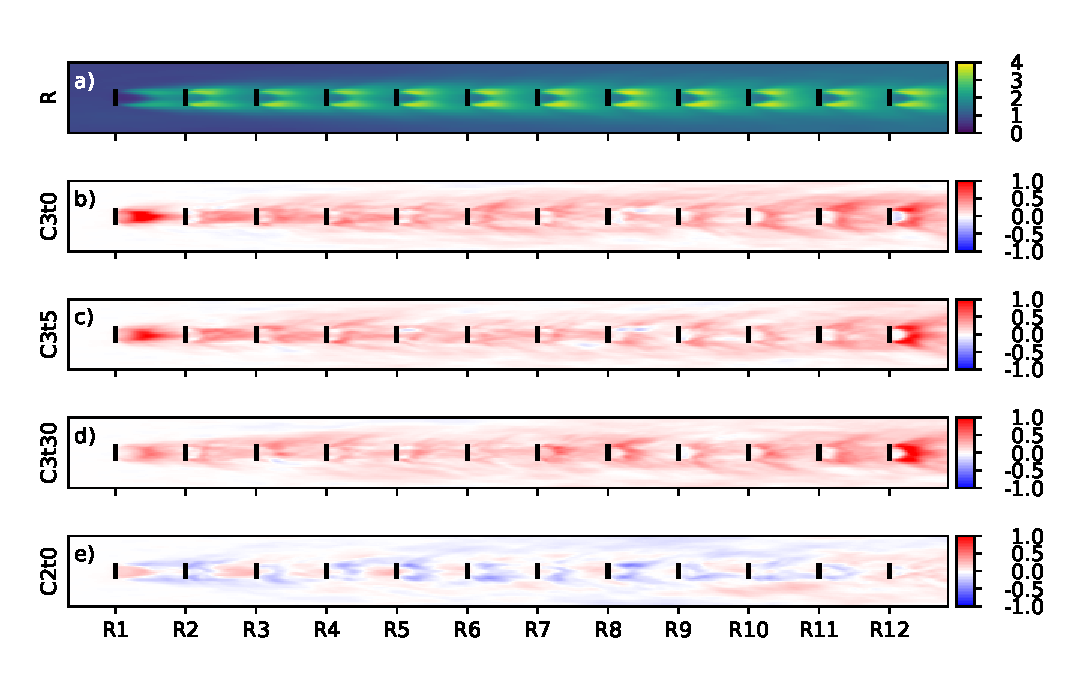
\includegraphics[width=0.93\textwidth]{chapters/optimal_induction_control/topview_tke.eps}
			\caption[Planview ($xy$) of \emph{turbulence} kinetic energy $k = (\overline{\widetilde{u}_x'\widetilde{u}_x'} + \overline{\widetilde{u}_y'\widetilde{u}_y'} + \overline{\widetilde{u}_z'\widetilde{u}_z'})/2$ at hub height.]{Planview ($xy$) of \emph{turbulence} kinetic energy $k = (\overline{\widetilde{u}_x'\widetilde{u}_x'} + \overline{\widetilde{u}_y'\widetilde{u}_y'} + \overline{\widetilde{u}_z'\widetilde{u}_z'})/2$ at hub height. \emph{a) } Reference case. \emph{b-e)} Difference between optimal control and reference case, defined as $\Delta = k_{\text{opt}} - k_{\text{R}}$  \label{fig:opt_ind_side_tke}}
		\end{figure}
	
		% SIDEVIEW U
		\begin{figure}[hbt]
			\centering
			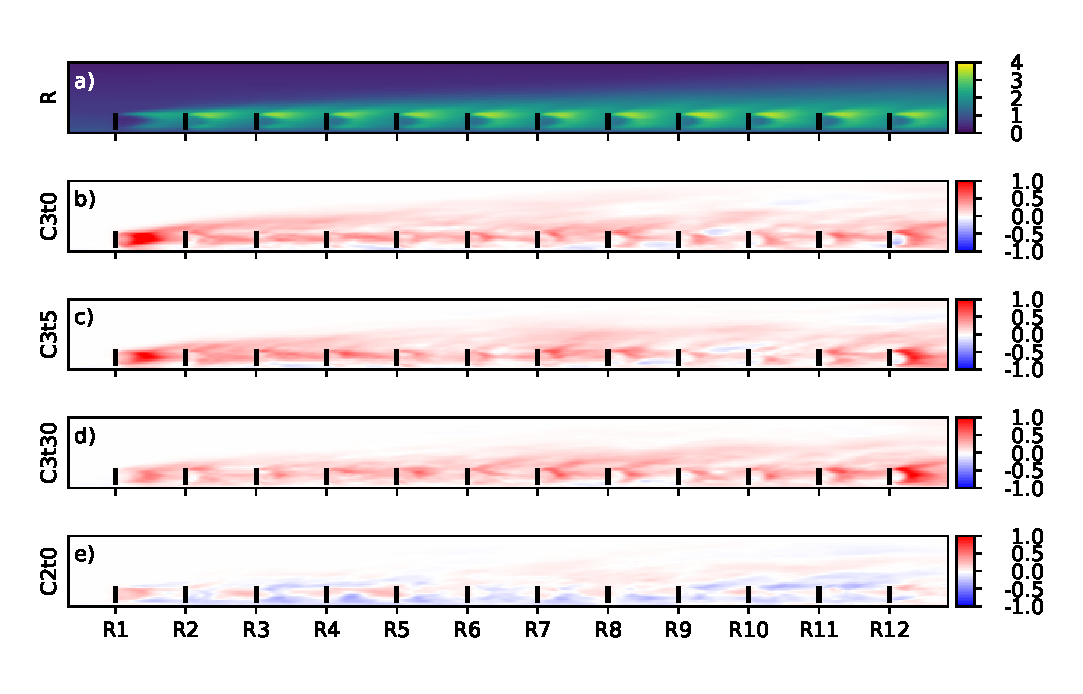
\includegraphics[width=0.93\textwidth]{chapters/optimal_induction_control/sideview_tke_side.eps}
			\caption[Sideview ($xz$) of \emph{turbulence} kinetic energy $k = \frac{1}{2}(\overline{\widetilde{u}_x'\widetilde{u}_x'} + \overline{\widetilde{u}_y'\widetilde{u}_y'} + \overline{\widetilde{u}_z'\widetilde{u}_z'})$ in turbine centerline plane.]{Sideview ($xz$) of \emph{turbulence} kinetic energy $k = \frac{1}{2}(\overline{\widetilde{u}_x'\widetilde{u}_x'} + \overline{\widetilde{u}_y'\widetilde{u}_y'} + \overline{\widetilde{u}_z'\widetilde{u}_z'})$ in turbine centerline plane. \emph{a) } Reference case. \emph{b-e)} Difference between optimal control and reference case, defined as $\Delta = k_{\text{opt}} - k_{\text{R}}$  \label{fig:opt_ind_top_tke}}
		\end{figure}

	\subsubsection{Transversal momentum transport}
	
		Figure~\ref{fig:opt_ind_top_uvm} shows planviews of  \emph{mean-flow} transversal transport of axial momentum $\widetilde{U}_x \widetilde{U}_y$ at hub height. The sign convention is such that positive values correspond to transport in the positive $y$ direction in the figure. As was the case in previous observations, cases C3t0 and C3t5 show similar behavior. Mean-flow transversal momentum transport into the wake region is increased significantly behind the first two turbine rows. Downstream of these rows, the difference between these cases and the reference case is far less coherent. The latter can be explained by the fact that it occurs in the region in which $\widetilde{U}_x$ in the intercolumn channels starts to deviate significantly from the reference case as shown in Figure~\ref{fig:opt_ind_top_u}. The wake region of the first row in case C3t30 shows a smaller increase in transversal transport into the wake, and the increased outwards transversal momentum transport at the turbine disk is likely to be caused by a higher mean value of $\cthat$. The opposite is true for the first-row turbine in case C2t0. No further coherent behavior can be identified from these latter two cases.
	
		% TOPVIEW UVM
		\begin{figure}[ht]
			\centering
			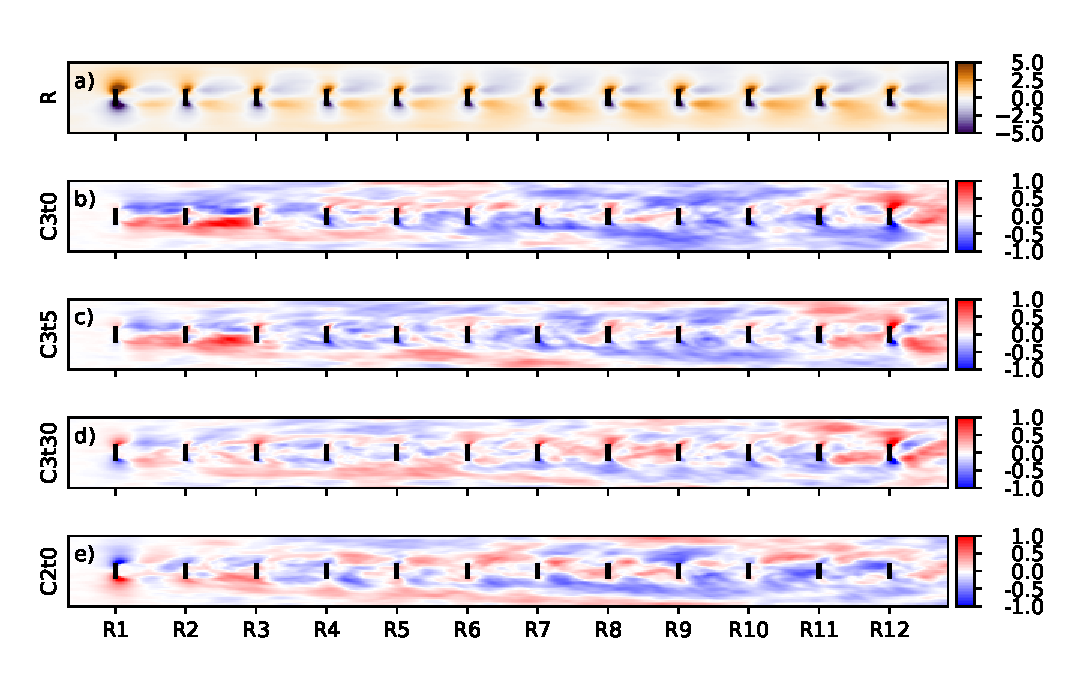
\includegraphics[width=0.92\textwidth]{chapters/optimal_induction_control/topview_uvm.eps}
			\caption[Planview ($xy$) of mean-flow transversal transport of axial momentum $\widetilde{U}_x \widetilde{U}_y$ at hub height.]{Planview ($xy$) of mean-flow transversal transport of axial momentum $\widetilde{U}_x \widetilde{U}_y$ at hub height. \emph{a) } Reference case. \emph{b-e)} Difference between optimal control and reference case, defined as $\Delta = (\widetilde{U}_x \widetilde{U}_y)_{\text{opt}} - (\widetilde{U}_x \widetilde{U}_y)_{\text{R}}$. \label{fig:opt_ind_top_uvm}}
		\end{figure}
	
		Figure~\ref{fig:opt_ind_top_uv} shows planviews of \emph{turbulent} transversal transport of axial momentum $\overline{\widetilde{u}_x' \widetilde{u}_y'}$ at hub height. For all overinductive cases an increased transport of momentum towards the wake centerline can be observed, whose effect is more pronounced for C3t0 and C3t5 than for C3t30. Note however that, although the absolute magnitude of this increased transport is about half that of the mean-flow transport in the first rows (Figure~\ref{fig:opt_ind_top_uvm}b,c), the relative increase over the reference value is similar for both mechanisms and constitutes about 25\%. Again, the underinductive case C2t0 shows no clearly coherent differences with the reference case. 
	
		% TOPVIEW UVturb
		\begin{figure}[hbt]
			\centering
			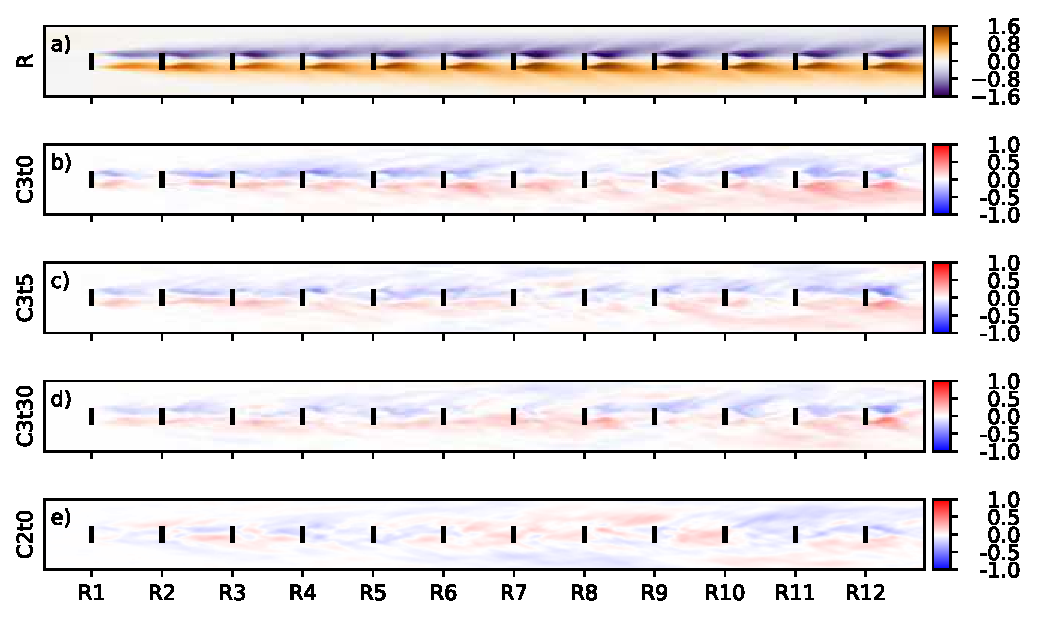
\includegraphics[width=0.92\textwidth]{chapters/optimal_induction_control/topview_uv.eps}
			\caption[Planview ($xy$) of turbulent transversal transport of axial momentum $\overline{\widetilde{u}_x' \widetilde{u}_y'}$ at hub height.]{Planview ($xy$) of turbulent transversal transport of axial momentum $\overline{\widetilde{u}_x' \widetilde{u}_y'}$ at hub height. \emph{a) } Reference case. \emph{b-e)} Difference between optimal control and reference case, defined as $\Delta = \overline{\widetilde{u}_x' \widetilde{u}_y'}_{\text{opt}} - \overline{\widetilde{u}_x' \widetilde{u}_y'}_{\text{R}}$  \label{fig:opt_ind_top_uv}}
		\end{figure}	
	
		\clearpage
	
	
	\subsubsection{Vertical momentum transport}

	Figure~\ref{fig:opt_ind_side_uwm} shows sideviews of \emph{mean-flow} vertical transport of axial momentum $- \widetilde{U}_x \widetilde{U}_z$ through the rotor centerline. The sign convention is such that downwards transport is positive. The figure illustrates virtually no differences between controlled and reference cases: the optimal control hence does not significantly influence the mean-flow top-down transport for any of the cases.

	% TOPVIEW UWM
	\begin{figure}[t]
		\centering
		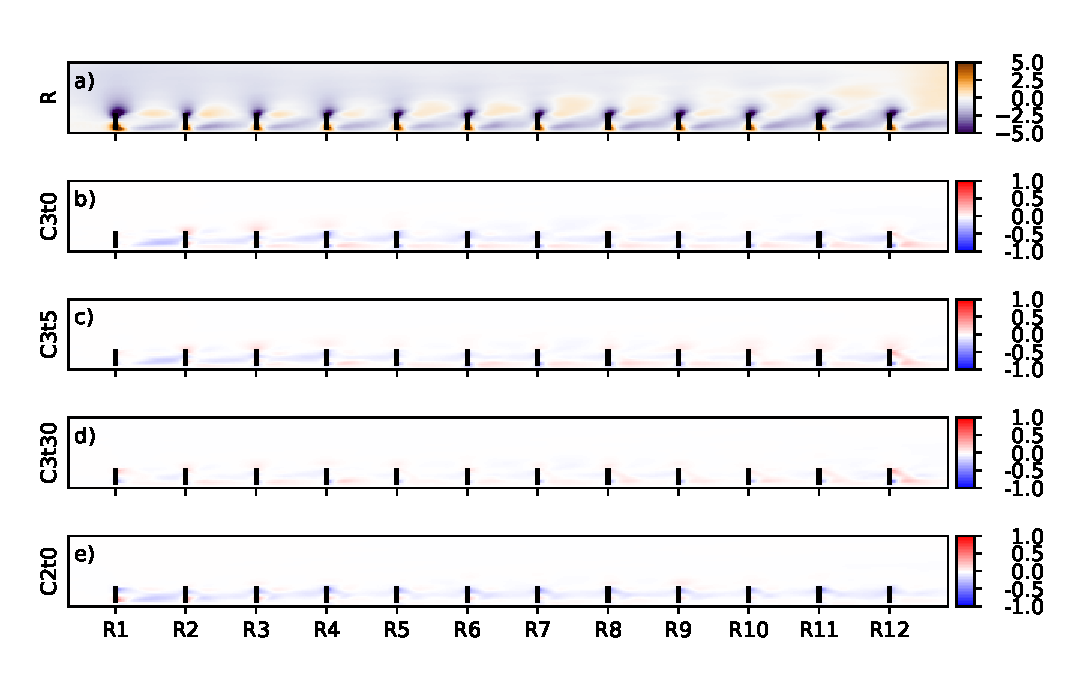
\includegraphics[width=0.93\textwidth]{chapters/optimal_induction_control/sideview_uwm.eps}
		\caption[Sideview ($xz$) of mean-flow top-down transport of axial momentum $- \overline{\widetilde{u}}_x~ \overline{\widetilde{u}}_z$ in turbine centerline plane.]{Sideview ($xz$) of mean-flow top-down transport of axial momentum $- \overline{\widetilde{u}}_x~ \overline{\widetilde{u}}_z$ in turbine centerline plane. \emph{a) } Reference case. \emph{b-e)} Difference between optimal control and reference case, defined as $\Delta = (- \overline{\widetilde{u}}_x~ \overline{\widetilde{u}}_z)_{\text{opt}} - (- \overline{\widetilde{u}}_x~ \overline{\widetilde{u}}_z)_{\text{R}}$. \label{fig:opt_ind_side_uwm}}
	\end{figure}

	Figure~\ref{fig:opt_ind_side_uw} shows sideviews of \emph{turbulent} vertical transport of axial momentum $- \overline{\widetilde{u}_x'\widetilde{u}_z'}$ through the rotor centerline. In contrast to the mean-flow transport described above, the turbulent transport shows significant deviations from the reference case: Throughout the wind-farm, all cases increase the turbulent entrainment of axial momentum at the interface between the wake and the flow above it. Similar to previous observations for other variables, this effect is most pronounced in the first row turbines of the overinductive case C3t0 and C3t5 (Figure\ref{fig:opt_ind_side_uw}b,c). Moreover, for these turbines, also a slight increase in upwards turbulent transport from underneath the rotor disk can be observed.

	% TOPVIEW UWturb
	\begin{figure}[bt]
		\centering
		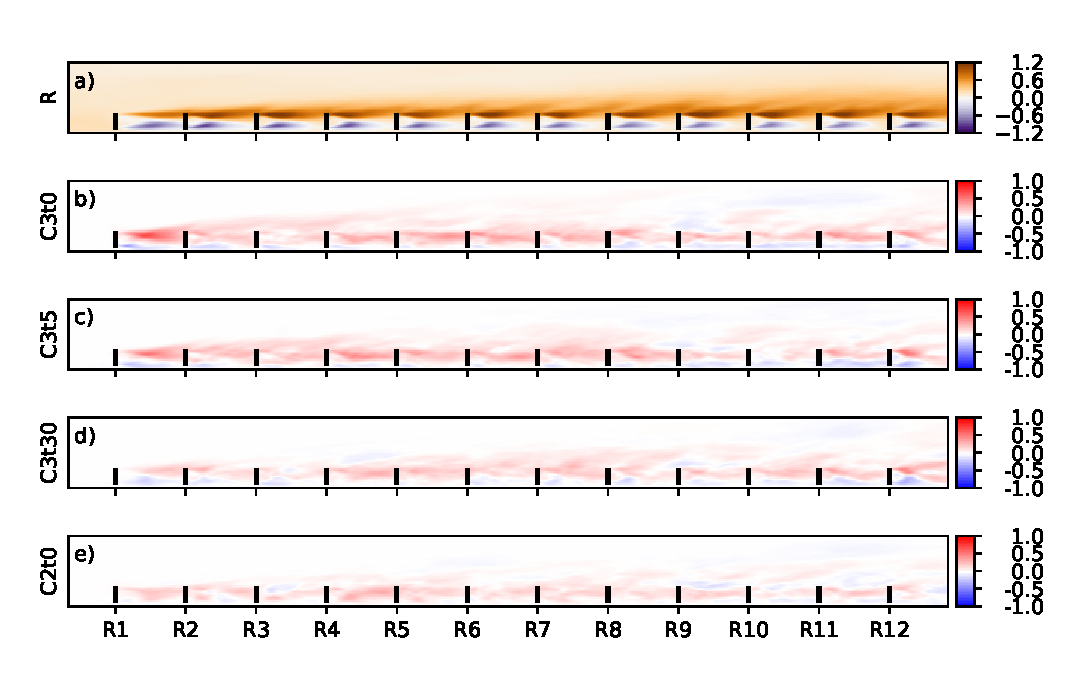
\includegraphics[width=0.93\textwidth]{chapters/optimal_induction_control/sideview_uw.eps}
		\caption[Sideview ($xz$) of turbulent top-down transport of axial momentum $- \overline{\widetilde{u}_x'\widetilde{u}_z'}$ in turbine centerline plane.]{Sideview ($xz$) of turbulent top-down transport of axial momentum $- \overline{\widetilde{u}_x'\widetilde{u}_z'}$ in turbine centerline plane. \emph{a) } Reference case. \emph{b-e)} Difference between optimal control and reference case, defined as $\Delta = (- \overline{\widetilde{u}_x'\widetilde{u}_z'})_{\text{opt}} - (- \overline{\widetilde{u}_x'\widetilde{u}_z'})_{\text{R}}$  \label{fig:opt_ind_side_uw}}
	\end{figure}	

	\subsubsection{Discussion}
	 A first observation that can be made across all control cases is the increase in mean axial velocity $\widetilde{U}_x$ at the turbine disks, as shown e.g. in Fig~\ref{fig:opt_ind_top_u}. Furthermore, for the overinductive cases C3t0, C3t5, and C3t30 a larger drop in $\widetilde{U}_x$ can be observed for many turbine rows, and the increase in velocity at the disks is hence caused by increased mixing and recovery as the wake progresses downstream. The underinductive case C2t0 however has higher $\widetilde{U}_x$ throughout the farm, which can be attributed to a lower mean thrust coefficient $\cthat$. 
	 
	 Throughout the observations, it was shown that case C3t0 and C3t5 show similar and coherent behavior, with C3t30 following the same trends to a lesser extent. Furthermore, many of the features seem to be most salient in the first row of turbines. In the remainder of the discussion, we will focus on the front row of the former two cases. The large increase in turbulence kinetic energy in the core region behind this row is consistent with a strongly enhanced wake recovery, as shown by the significant increase in axial velocity in the regions just downstream of this core (Figure~\ref{fig:opt_ind_top_u}b,c and Figure~\ref{fig:opt_ind_side_u}b,c). These observations explain the large gains in power extraction for these rows shown in Figure~\ref{fig:bar_and_row}. Upon investigating the origins of this enhanced recovery, it was found that the mean-flow transport of axial momentum $\widetilde{U}_x \widetilde{U}_y$ from the entrance region of the intercolumn channels towards the wake centerline was significantly enhanced by the optimal control. Further, the \emph{relative} increase in turbulent transport $\overline{\widetilde{u}_x' \widetilde{u}_y'}$ constitutes about 25$\%$ of the reference value, similar to the increase in mean-flow transversal transport. This increase in turbulent transport was also seen in downstream regions of the farm, whereas the mean-flow transport behavior is clouded by overall deceleration of the mean flow in the intercolumn channels. Turning to the \emph{vertical} transport, it was found that mean-flow transport $-\widetilde{U}_x \widetilde{U}_z$ was unaffected, whereas top-down turbulent entrainment $- \overline{\widetilde{u}_x' \widetilde{u}_z'}$ is enhanced throughout the wind farm. 

\section{Summary}\label{sec:opt_ind_summ}
In this chapter, the optimal coordinated axial induction control of an aligned wind farm with $12 \times 6$ turbines was investigated. A suite of control cases was defined, based on differing wind turbine response times and whether or not overinduction was allowed. All control cases, except for the most restrictive one, showed an increase in wind-farm energy extraction ranging from 8 to 21$\%$. Further, it was shown that also cases with smooth turbine dynamics are able to sustain significant power increases. Finally, the wind-farm flow field statistics of the optimal control simulations were analyzed and compared to the reference case. It was found that all cases experience higher disk velocities throughout the wind farm. Further, the most coherent behavior could be identified in the overinductive cases C3t0 and C3t5, for which turbulence kinetic energy and turbulent momentum transport towards the wake center were observed. Furthermore, increased transversal mean-flow transport was found in the entrance region of the wind farm. In this chapter, we analyzed and observed the effects of the optimal controls on the flow field statistics that result in an overall aggregated wind-farm power increase. However, the question of \emph{how} these changes to the flow field are constituted by the optimal controls still remains unanswered. This is further discussed in the next chapter. 

\cleardoublepage
